% pdflatex paper.tex
% biber paper.bcf
% pdflate paper.tex (x2)

\documentclass[twoside]{article}

\usepackage[sc]{mathpazo}
\usepackage[utf8]{inputenc}
\usepackage[english,italian]{babel}
\linespread{1.05} % Line spacing - Palatino needs more space between lines
\usepackage{microtype} % Slightly tweak font spacing for aesthetics

\usepackage{graphicx}
\usepackage[hmarginratio=1:1,top=32mm,columnsep=20pt, margin=2.5cm]{geometry} % Document margins
%\usepackage{multicol} % Used for the two-column layout of the document
\usepackage[hang, small,labelfont=bf,up,textfont=it,up]{caption} % Custom captions under/above floats in tables or figures
\usepackage{booktabs} % Horizontal rules in tables
\usepackage{float} % Required for tables and figures in the multi-column environment - they need to be placed in specific locations with the [H] (e.g. \begin{table}[H])
\usepackage{hyperref} % For hyperlinks in the PDF
\usepackage{listings}

\usepackage{lettrine} % The lettrine is the first enlarged letter at the beginning of the text
\usepackage{paralist} % Used for the compactitem environment which makes bullet points with less space between them

%\usepackage{geometry} % Impostazioni margini
%\geometry{a4paper,top=3cm,bottom=3cm,left=1.30cm,right=1.30cm,%
%    heightrounded,bindingoffset=5mm}
    
\usepackage{textcomp} % Impostazioni codici
\usepackage[T1]{fontenc}
\lstset{
  basicstyle=\ttfamily,
  columns=flexible,
  upquote,
}

\usepackage{forest} % Usare system-tree

\usepackage{abstract} % Allows abstract customization
\renewcommand{\abstractnamefont}{\normalfont\bfseries} % Set the "Abstract" text to bold
\renewcommand{\abstracttextfont}{\normalfont\small\itshape} % Set the abstract itself to small italic text

\usepackage{titlesec} % Allows customization of titles
\renewcommand\thesection{\Roman{section}} % Roman numerals for the sections
\renewcommand\thesubsection{\Roman{subsection}} % Roman numerals for subsections
\titleformat{\section}[block]{\large\scshape\centering}{\thesection.}{1em}{} % Change the look of the section titles
\titleformat{\subsection}[block]{\large}{\thesubsection.}{1em}{} % Change the look of the section titles
%\usepackage{fancyhdr} % Headers and footers
%\pagestyle{fancy} % All pages have headers and footers
%\fancyhead{} % Blank out the default header
%\fancyfoot{} % Blank out the default footer
%\fancyhead[C]{$\bullet$ Gennaio 2016 $\bullet$} % Custom header text
%\fancyfoot[RO,LE]{\thepage} % Custom footer text

\usepackage{amsmath}
\usepackage{txfonts}
\usepackage{enumitem}

\usepackage{subcaption}

\usepackage{biblatex}
\bibliography{bibliography}

\setlength\parindent{0pt} % Nessuna rientranza ad inizio paragrafo
\setlength\parskip{10pt} % Spaziatura tra paragrafi

% Impostazioni system-tree
%\definecolor{folderbg}{RGB}{124,166,198}
%\definecolor{folderborder}{RGB}{110,144,169}
%
%\def\Size{4pt}
%\tikzset{
%  folder/.pic={
%    \filldraw[draw=folderborder,top color=folderbg!50,bottom color=folderbg]
%      (-1.05*\Size,0.2\Size+5pt) rectangle ++(.75*\Size,-0.2\Size-5pt);  
%    \filldraw[draw=folderborder,top color=folderbg!50,bottom color=folderbg]
%      (-1.15*\Size,-\Size) rectangle (1.15*\Size,\Size);
%  }
%}

%----------------------------------------------------------------------------------------
% IMPOSTAZIONI DI SILLABAZIONE
%----------------------------------------------------------------------------------------

\hyphenation{dynamo baseball cluster consistency COPS replication availability partition-tolerance Communications SIGOPS annual preserving performance verificaDisponibilitaMagazzino}
% Inserire le parole che non devono essere sillabate e spezzate da tex

%----------------------------------------------------------------------------------------
%	CUSTOM MACRO
%----------------------------------------------------------------------------------------

\newcommand{\vclock}{\mathrm{VC}} % VC

%----------------------------------------------------------------------------------------
%	TITLE SECTION
%----------------------------------------------------------------------------------------

\title{\vspace{-15mm}\fontsize{24pt}{10pt}\selectfont\textbf{Ingegneria del Software Orientata ai Servizi: relazione di progetto}} % Article title

\author{
\large
\textsc{Bartolomeo Lombardi, Amerigo Mancino, Andrea Segalini}\\[2mm] % Your name
\normalsize Università degli Studi di Bologna % Your institution
\vspace{5mm} \\
\normalsize \href{mailto:bartolomeo.lombardi@studio.unibo.it}{bartolomeo.lombardi@studio.unibo.it}\\
\normalsize \href{mailto:amerigo.mancino@studio.unibo.it}{amerigo.mancino@studio.unibo.it}\\
\normalsize \href{mailto:andrea.segalini@studio.unibo.it}{andrea.segalini@studio.unibo.it}
\vspace{-5mm}
}
\date{Anno Accademico 2015-16}

%----------------------------------------------------------------------------------------

\begin{document}
\maketitle 
%\thispagestyle{fancy} % All pages have headers and footers

%----------------------------------------------------------------------------------------
%	ABSTRACT
%----------------------------------------------------------------------------------------

\begin{abstract}
\noindent
Costruire sistemi software è un lavoro complesso. Costruire grandi sistemi software facendo interagire
diverse componenti che appartengono ad organizzazioni differenti è ancora più complesso. I servizi e i
processi sono le astrazioni che l'Ingegneria del Software insegna ad usare per affrontare questa
complessità.
In questa relazione descriveremo la progettazione e realizzazione delle attività di ACME, un'azienda
che si occupa della fornitura e dell'assemblaggio di biciclette, compresi i relativi accessori. Verranno
analizzate nel dettaglio tutte le fasi di modellazione affrontate, a partire dalla descrizione
dei processi di ACME mediante un BPMS, fino ad arrivare all'esposizione esaustiva di alcune capability
esterne implementate mediante API REST. Verranno inoltre discusse le difficoltà incontrate e saranno
mostrati gli espedienti che hanno portato alla loro risoluzione.
\end{abstract}

%----------------------------------------------------------------------------------------

\vspace{15mm} % Spaziatura tra abstract e corpo articolo %% backup {20mm}

\section{Introduzione: tecnologie utilizzate}
In questo paragrafo verranno brevemente descritte le principali tecnologie utilizzate
durante la realizzazione del progetto:
\begin{itemize}
	\item Camunda \\
		  Piattaforma open-source per la gestione di processi business e di diagrammi di flusso,
		  oltre che per l'orchestrazione dei servizi,
		  usata principalmente, nel nostro caso, per la simulazione di human workflow.
	\item Jolie \\
		  Linguaggio di programmazione ``orientato ai servizi'' in grado di supportare la nozione
		  di \textit{operation} e che facilita la comunicazione fra processi ed entità differenti.
	\item Signavio Process Editor \\
		  Lanciato nel Maggio del 2009, è un tool completamente gratuito e web-based per la
		  modellazione di processi business.
	\item HSQLDB \\
		  Scritto principalmente in Java e sviluppato da HSQLDB Developer Group, è un RDBMS
		  rilasciato con licenza libera e completamente compatibile con Jolie che può essere
		  usato sia come server che come istanza interna ad un'applicazione.
	\item JAX-WS \\
		  Java API for XML Web Services è un insieme di procedure (API) del linguaggio di programmazione
		  Java dedicate allo sviluppo di servizi web, che ci sono servite, ad esempio, nell'implementazione
		  dei web services client e server in Java.
\end{itemize}

\section{Interpretazione della specifica}
L'azienda ACME si occupa di fornire biciclette assemblate su richiesta ed accessori
a rivendite che operano direttamente con il pubblico.
Gli accessori e i componenti sono stati intesi genericamente come ``pezzi'', i quali possono
essere ``assemblabili'', ossia montati nel magazzino principale, oppure ``non assemblabili'',
ossia spediti direttamente alle rivendite e quindi venduti separatamente o montati in loco.
Per esempio, abbiamo considerato il pezzo ``ruota'' come assemblabile mentre il pezzo ``campanello''
come non assemblabile.
In prima approssimazione, ad ACME giungono degli ordini costituiti da liste di pezzi,
ognuno dei quali è rappresentato con il codice prodotto e con la quantità richiesta.
Quando viene ricevuto un ordine, l'azienda controlla che i pezzi siano compatibili tra loro
e che siano presenti tutti quelli indispensabili per la costruzione della bicicletta. In caso
negativo, un impiegato notifica al cliente il problema e lo invita a ripetere dall'inizio l'ordine,
il quale viene abortito, terminando il processo.
In caso positivo, invece, il processo procede verificando la disponibilità dei pezzi come segue:
\begin{enumerate}
	\item Si controlla se i pezzi sono presenti già nel magazzino principale.
	\item Per tutti quelli non presenti, vengono contattati tutti i magazzini secondari e
		  recuperate le informazioni.
	\item Qualora ci fossero ancora pezzi mancanti, viene contattato un fornitore esterno
		  ad ACME.
\end{enumerate}
Al termine di questa fase di controllo, otteniamo una tabella contenente, per ogni pezzo, le informazioni sul
magazzino che lo possiede e in quale quantità. Nel caso del fornitore esterno, recuperiamo anche
il prezzo di vendita. Queste informazioni saranno anche utilizzate per determinare, per ogni pezzo non
assemblabile, il magazzino geograficamente più vicino al cliente che si preoccuperà della spedizione
tramite un corriere. Se, al termine di questa procedura, dovessero esserci dei pezzi mancanti
(non disponibili), si avviserà il cliente di tale problema e il processo verrà abortito senza
possibilità di soluzione. \newline
Riguardo i pezzi non assemblabili, per ogni pezzo viene eseguito un ordinamento basato sulla distanza
dei magazzini che lo posseggono dal cliente e vengono scelti i magazzini più vicini, fino ad esaurire la
quantità richiesta. Ad esempio, se vengono richiesti due campanelli e il magazzino più vicino al cliente
ne possiede uno solo, quest'ultimo si preoccupa di spedire l'oggetto nella quantità che possiede e i
restanti sono gestiti dal successivo magazzino nella graduatoria. \newline
Nel caso in cui tutti i pezzi siano disponibili in qualche modo, viene preparato un preventivo e valutata
l'applicazione di uno sconto. Indi, viene inviata la proposta di pagamento al cliente, il quale
ha cinque giorni di tempo per accettare o rifiutare l'offerta. In caso di diniego, il processo termina. In caso
di accettazione, invece, il cliente invia un riferimento alla ricevuta del versamento di un anticipo
verso ACME. Abbiamo ipotizzato che l'azienda verifichi periodicamente se il pagamento è stato
effettuato, chiedendo conto alla banca. Se, dopo tre giorni, l'accredito non dovesse essere ancora pervenuto,
l'intero ordine viene annullato. \newline
Nella fase successiva, è necessario riservare tutti i pezzi in maniera tale da evitare possibili conflitti
fra ordini concorrenti. Questa operazione avviene come se fosse una transazione, ossia tutti i pezzi vengono
giustamente riservati, oppure vengono disfatte tutte le prenotazioni di quell'ordine già effettuate e l'ordine
stesso viene cancellato.
In parallelo si contattano tutti i magazzini secondari, il magazzino principale e il fornitore esterno.
Se, alla fine, tutti i pezzi sono stati correttamente riservati, si notifica ad ognuno dei magazzini e
al supplier di procedere alla spedizione, mediante un corriere.
In base al pezzo, la spedizione è divisa in due gruppi: una con destinazione il cliente e/o
una con destinazione il magazzino principale. 
Da questo momento in poi l'ordine non potrà più essere annullato. \newline
In seguito, il magazzino principale riceve parallelamente da tutte le sedi secondarie i vari componenti
e procede con l'assemblaggio e la spedizione del prodotto finale. Quindi, ACME rimane in attesa
della ricevuta da parte del cliente dell'avvenuto pagamento restante. La verifica avviene contattando
la banca nella stessa modalità esposta in precedenza. Se, dopo tre giorni, l'accredito non dovesse essere
ancora pervenuto, l'amministrazione dell'azienda si attiva per prendere i dovuti provvedimenti.
In ogni caso, a questo punto, il processo termina.

\section{SOA modeling} \label{soa_modeling}
In questo paragrafo descriveremo brevemente le capabilities offerte dal sistema, con
particolare enfasi a quelle che sono state maggior oggetto di studio durante l'elaborazione
del progetto.
Il nostro business espone all'utente una sola capability, che avvia
il processo di costruzione e consente di effettuare un ordine.
Il magazzino principale si occupa della coordinazione di tutti i magazzini secondari (compresa la
parte operativa di sé stesso) e, pertanto, deve essere capace di:
\begin{itemize}
	\item Mandare richieste di
		  ``verifica disponibilità'' verso tutti i magazzini secondari e presso un eventuale
		  fornitore esterno.
	\item Mandare richieste di ``riserva pezzi''
		  a tutti i magazzini secondari e presso un eventuale fornitore esterno.
	\item Mandare richieste di
		  ``elimina pezzi'' verso tutti i magazzini secondari e presso un eventuale fornitore
		  esterno.
	\item Eseguire l'ordine, informando i magazzini secondari di procedere alla spedizione dei diversi pezzi
	   	  richiesti (se necessario), mettendosi poi in attesa delle varie consegne.
	\item Assemblare il ciclo e preparare il tutto per la spedizione.
\end{itemize}
Come si vede, il magazzino principale è quindi composto da una parte, appunto, ``principale'', che
funge da coordinatore, e da un magazzino secondario.
In aggiunta, un generico magazzino secondario deve poter:
\begin{itemize}
	\item Verificare la disponibilità dei pezzi e recuperare le informazioni a riguardo
		  per il suo magazzino.
	\item Riservare i pezzi presso il suo magazzino.
	\item Eliminare la prenotazione di determinati pezzi presso il suo magazzino.
	\item Eseguire l'ordine, che comporta l'invio dei pezzi verso il magazzino principale
		  oppure direttamente verso l'utente affidandosi ad un corriere esterno.
\end{itemize}
L'amministrazione, a sua volta, deve essere in grado di:
\begin{itemize}
	\item Creare una nuova istanza dell'ordine.
	\item Verificare la compatibilità di pezzi.
	\item Calcolare le distanze fra due punti geografici.
	\item Chiedere alla banca se un certo ammontare è stato pagato da un cliente.
	\item Verificare i pagamenti, contattando la banca.
	\item Trovare il miglior magazzino per ogni pezzo dell'ordine.
\end{itemize}
Sappiamo anche che il fornitore esterno, nonostante non faccia parte del nostro business,
è capace di:
\begin{itemize}
	\item Verificare la disponibilità dei pezzi e recuperare le informazioni disponibili a riguardo.
	\item Riservare i pezzi richiesti da ACME.
	\item Eliminare la prenotazione di determinati pezzi.
	\item Eseguire l'ordine, spedendo i pezzi richiesti al magazzino principale di ACME.
\end{itemize}
Chiaramente alcune delle capabilities qui esposte sono state accorpate per essere implementate
come un unico servizio offerto all'utente.

La nostra SOA, quindi, è formata da tre servizi fondamentali: l'amministrazione, il magazzino principale e un
servizio di magazzino secondario. La prima espone come operation al cliente una sola capability
che consente di effettuare l'ordine e di ricevere il prodotto finale.
Le altre capabilities amministrative non vengono esposte sotto forma di operations
ma sono integrate nell'applicazione e non rese accessibili all'esterno.
Sia il servizio magazzino principale che il secondario implementano tutte le capabilities sopra indicate.

Illustriamo brevemente in figura \ref{fig:4} le interazioni fra le varie componenti del sistema.

\begin{figure}[!tbp]
\centering
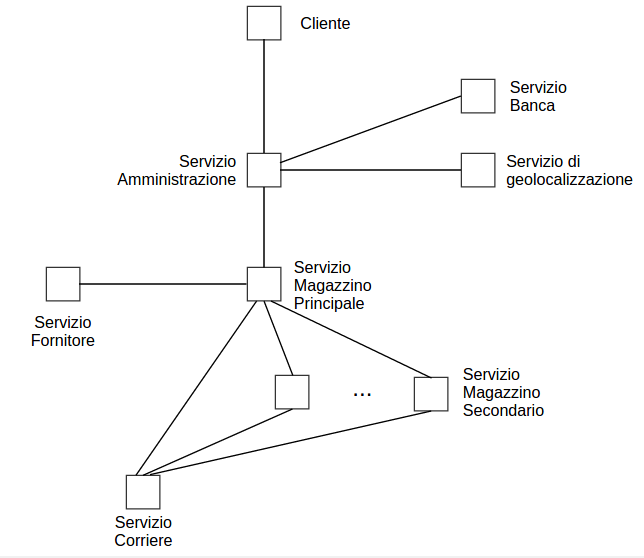
\includegraphics[width=9cm]{schema.png}
\caption{Schema delle interazioni fra componenti del sistema.}\label{fig:4}
\end{figure}

\section{Implementazione dei servizi}
In questo paragrafo tratteremo delle scelte implementative che abbiamo preso nella realizzazione
della nostra SOA, descrivendo anche i web service server implementati con Jolie.
Abbiamo definito due applicativi principali che espongono le capabilities del magazzino principale
(amministrazione e coordinazione) e secondario (parte operativa). 

\lstset{frame=trBL}

\subsection{Magazzino principale}
Realizzato in Jolie, l'interfaccia del servizio è descritta di seguito:

\begin{lstlisting}
include "dataTypes.iol"

interface InterfacciaMagazzinoPrincipale {
  RequestResponse:
    verificaDisponibilitaMagazzini(RichiestaOrdine)(RispostaVerificaDisponibilita),
    verificaDisponibilitaMagazzino(RichiestaMagazzino)(RispostaMagazzino),
    verificaDisponibilitaFornitore(RichiestaFornitore)(RispostaFornitore),

    prenotaPezziMagazzini(RichiestaPrenotazioneMagazzini)(PezziMancanti),
    prenotaPezziMagazzino(RichiestaPrenotazioneMagazzino)(PezziMancanti),
    prenotaPezziFornitore(RichiestaPrenotazioneFornitore)(PezziMancanti),

    creaIstanzaOrdine(RichiestaCreaOrdine)(void),
  
    eliminaPrenotazioneMagazzini(RichiestaEliminazioneMagazzini)(void),
    eliminaPrenotazioneMagazzino(RichiestaEliminazioneMagazzino)(void),
    eliminaPrenotazioneFornitore(RichiestaEliminazioneFornitore)(void),

    eseguiOrdineMagazzini(RichiestaEsecuzioneMagazzini)(void),
    eseguiOrdineMagazzino(RichiestaEsecuzioneMagazzino)(void),
    eseguiOrdineFornitore(RichiestaEsecuzioneFornitore)(void),
    
    assemblaCiclo(RichiestaAssembla)(void)
}
\end{lstlisting}

dove \textit{dataTypes.iol} è il file contenente le definizioni di tutti i tipi di dato scambiati
durante l'invocazione delle operazioni. Il magazzino principale funge, dunque, da coordinatore
di tutti i magazzini secondari, verificando la disponibilità dei pezzi, prenotandoli o eliminandoli
da un ordine esistente. I magazzini secondari, che descriveremo nel dettaglio in seguito,
rappresentano invece la parte operativa di un magazzino, ossia possiedono unicamente la capacità
di memorizzare le quantità di pezzi da loro posseduti, gli ordini (lotti di pezzi da recapitare
al cliente), etc.
Le operations di questa interfaccia sono esposte attraverso
la porta Jolie \textit{MagazzinoPrincPort}:

\begin{lstlisting}
inputPort MagazzinoPrincPort {
  Location: "socket://localhost:8000"
  Protocol: soap {
    .wsdl = "file:magazzinoPrincipale.wsdl";
    .wsdl.port = "MagazzinoPrincServicePort";
    .dropRootValue = true
  }  
  Interfaces: InterfacciaMagazzinoPrincipale
}
\end{lstlisting}

La porta utilizza il protocollo SOAP e il suo corrispondente WSDL è stato generato mediante il comando:

\begin{lstlisting}
$ jolie2wsdl -i ~/Scrivania/interfacce/:/usr/lib/jolie/include/ \
  -namespace org.acme.magazzino-principale -portName MagazzinoPrincPort \
  -portAddr http://localhost:8000 \
  -o magazzinoPrincipale.wsdl magazzinoPrincipale.ol
\end{lstlisting}

Il servizio comunica con le altre entità attraverso le seguenti output port:

\begin{lstlisting}
outputPort ServizioMagazzinoPrincipale {
  Location: "socket://localhost:8000"
  Protocol: soap 
  Interfaces: InterfacciaMagazzinoPrincipale
}
\end{lstlisting}

\textit{ServizioMagazzinoPrincipale} consente al magazzino di comunicare con sé stesso, in
quanto operations come la \texttt{verificaDisponibilitaMagazzini}, ad esempio,
richiama, per tutti gi $n$ magazzini secondari, l'operazione di \newline
\texttt{verificaDisponibilitaMagazzino}. La prima, infatti, si occupa di invocare la seconda
per ogni magazzino gestito da ACME, mettendo poi insieme le informazioni ricavate mentre la 
\texttt{verificaDisponibilitaMagazzino} permette di contattare immediatamente il magazzino stabilito.
Le altre operations che si occupano di eseguire l'ordine, prenotare i pezzi o eliminare una
prenotazione funzionano pressappoco nella stessa maniera.
Nel database registriamo tutte le informazioni necessarie per gestire la molteplicità di magazzini
secondari, ossia, in breve:
\begin{itemize}
	\item Un identificatore opportuno.
	\item L'URL del servizio magazzino secondario (nota: questo approccio molto naive è stato
		  adottato per semplicità, evitando di addentrarsi in strumenti per la gestione del
		  naming).
	\item Un booleano che identifica se si tratta di un fornitore esterno oppure di un
		  magazzino interno (nota: anche i fornitori vengono memorizzati insieme ai
		  magazzini secondari per semplicità).
\end{itemize}

Mediante questo stratagemma, riusciamo a ridurre la complessità del codice.
La altre porte:

\begin{lstlisting}
outputPort ServizioMagazzinoSecondario {
  Protocol: soap
  Interfaces: InterfacciaMagazzinoSecondario
}

outputPort ServizioFornitore {
  Protocol: soap
  Interfaces: InterfacciaFornitore
}
\end{lstlisting}

non possiedono la direttiva di \textit{location}, dal momento che viene impostata dinamicamente
prima di una chiamata in base ai magazzini secondari presenti nel database. Nel codice
mostrato di seguito notiamo come in \texttt{tabellaMagazzini} sono presenti le informazioni
dei magazzini e, in questo caso, il campo \texttt{url} viene assegnato al campo
\texttt{location} della porta \texttt{ServizioMagazzinoSecondario}:
\begin{lstlisting}
ServizioMagazzinoSecondario.location = tabellaMagazzini.(idMagazzino).url;
\end{lstlisting}
Sottolineiamo la presenza di un file di configurazione che, nel nostro intento originario,
doveva servire per impostare i parametri di deployment (location e port). Tuttavia in Jolie
è possibile settare tali parametri solo staticamente. Questo file è stato utilizzato allora
principalmente per caricare i dati relativi alla connessione con il DB (utente e password, driver,
porta, url, etc). Il database è gestito da HSQLDB \footnote{Sito web \url{www.hsqldb.org}},
scelto poiché consigliato dalla documentazione ufficiale di Jolie. La sua struttura è descritta
dal diagramma mostrato di seguito:

\begin{figure}[!htbp]
\centering
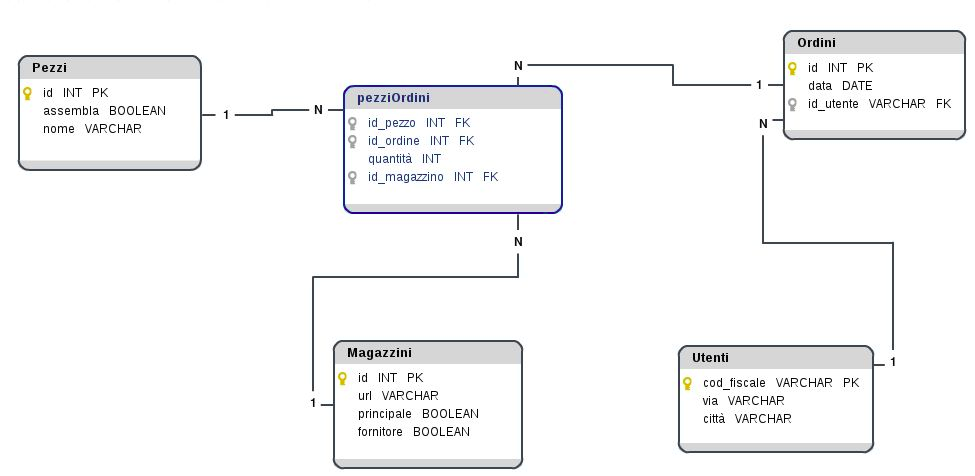
\includegraphics[width=13cm]{modello_logico_mag_principale.png}
\label{fig:3}
\end{figure}
\newpage
Ribadiamo che, la tabella \texttt{pezzi}, nel caso del magazzino principale, funge da ``catalogo''
dell'intera collezione di oggetti che ACME dispone e non è a conoscenza della quantità posseduta
dai magazzini secondari. In aggiunta, è necessario memorizzare anche le informazioni relative
all'utente, dal momento che il fornitore esterno necessita di sapere l'indirizzo di eventuali spedizioni
di pezzi non assemblabili.

\subsection{Magazzino secondario}
Il servizio magazzino secondario, realizzato anch'esso in Jolie, implementa tutte le
capabilities esposte nel paragrafo \ref{soa_modeling}.
La sua interfaccia è mostrata di seguito:
\begin{lstlisting}
include "dataTypes.iol"

interface InterfacciaMagazzinoSecondario {
  RequestResponse:
    verificaDisponibilitaPezzi(RichiestaDisponibilitaPezzi)(RispostaMagazzinoSecondario),
    prenotaPezzi(RichiestaPrenotazionePezzi)(PezziMancanti)
  
  OneWay:
    eliminaPrenotazionePezzi(int),
    eseguiOrdinePezzi(int) 
}
\end{lstlisting}
Il magazzino secondario si occupa della verifica della presenza di pezzi al suo interno,
oltre che della spedizione dei suddetti pezzi verso il magazzino principale oppure
direttamente verso il cliente. Il servizio è esposto attraverso la porta Jolie:
\begin{lstlisting}
inputPort MagazzinoSecPort {
  Location: "socket://localhost:8002"
  Protocol: soap
  Interfaces: InterfacciaMagazzinoSecondario
}
\end{lstlisting}
Per il magazzino secondario valgono all'incirca le stesse considerazioni fatte nel
paragrafo precedente. Di questo servizio non è stato generato un WSDL poiché, allo
stato attuale, serve unicamente il magazzino principale (scritto anch'egli in Jolie, come
già detto).
Inoltre, poggia anch'esso su un datatabase, la cui struttura è mostrata di seguito:

\begin{figure}[!htbp]
\centering
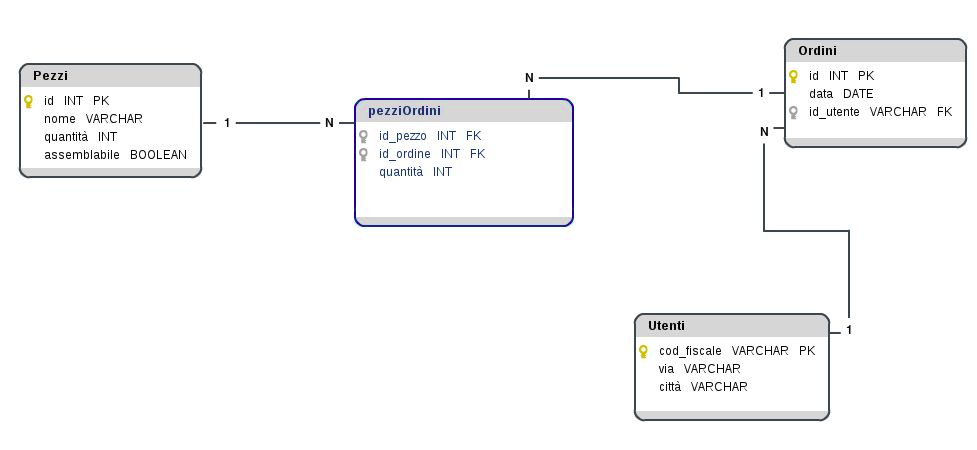
\includegraphics[width=13cm]{modello_logico_magazzino2.png}
\label{fig:2}
\end{figure}

In questo caso, la tabella \texttt{pezzi} contiene le informazione relative ai diversi
componenti posseduti dal magazzino fisico, compresa la quantità. I dati sugli utenti sono
necessari per il recapito di un'eventuale spedizione. Notiamo che i magazzini secondari
non memorizzano informazioni sugli altri.

\subsection{Amministrazione}
Il servizio di amministrazione espone come operations l'intero processo business di ordine
e assemblaggio del ciclo e funge, quindi, da orchestratore dell'applicazione, richiamando
le operations delle altre componenti quando opportuno. \`E stato implementato utilizzando Camunda
\footnote{Sito web \url{www.camunda.org}}, un BPMS che funge da execution engine per un
diagramma BPMN, offrendo di default un'interfaccia grafica per la parte di human workflow.

In questo progetto, è stata realizzata una parte del diagramma dell'amministrazione,
riportata di seguito:

\begin{figure}[!htbp]
\centering
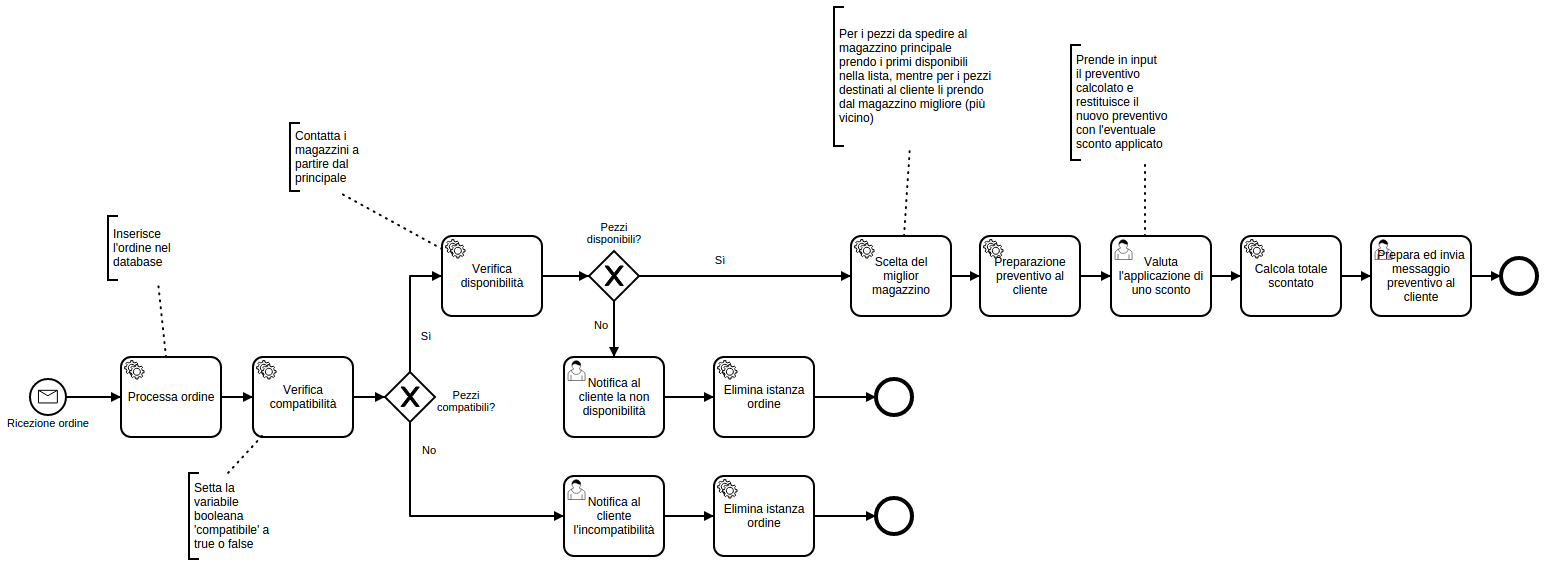
\includegraphics[width=17cm]{screen-bpmn-camunda.png}
\label{fig:bpmn}
\end{figure}

Le service task sono state realizzate attraverso una classe Java che implementa l'interfaccia
\texttt{JavaDelegate}. Il codice presente all'interno del metodo \texttt{execute} sarà quello
eseguito dall'execution engine durante l'avanzamento del flusso.

Nel processo vengono invocate operations di web services attraverso Java e l'utilizzo di JAX-WS.
In particolare, è stata utilizzata l'implementazione presente in Apache CXF
\footnote{Sito web \url{www.cxf.apache.org}}, con il quale sono state generate, partendo dal WSDL
del magazzino principale, delle classi Java. Tra queste è presente la rappresentazione
dei tipi di dati scambiati durante le invocazioni e il proxy per effettuare le chiamate.

Per la generazione, è stato necessario aggiungere al file \texttt{pom.xml}
il plugin di CXF, modificando WSDL e relativa location:
\begin{lstlisting}
<plugin>
      <groupId>org.apache.cxf</groupId>
      <artifactId>cxf-codegen-plugin</artifactId>
      <version>3.1.4</version>
      <executions>
          <execution>
              <id>generate-sources</id>
              <phase>generate-sources</phase>
              <configuration>
                  <sourceRoot>${project.build.directory}/generated/cxf</sourceRoot>
                  <wsdlOptions>
                      <wsdlOption>
                          <wsdl>${basedir}/src/main/resources/magazzinoPrincipale.wsdl</wsdl>
                          <wsdlLocation>classpath:magazzinoPrincipale.wsdl</wsdlLocation>
                      </wsdlOption>
                  </wsdlOptions>
              </configuration>
              <goals>
                  <goal>wsdl2java</goal>
              </goals>
          </execution>
      </executions>
</plugin>
\end{lstlisting}

Il processo viene attivato dalla ricezione di un messaggio SOAP che invoca l'operation di ``faiOrdine''.
I parametri del messaggio sono i dati dell'utente e l'ordine (lista dei pezzi con relativa quantità).
Questi ultimi sono rappresentati dalle classi autogenerate \texttt{Utente} e \texttt{List<Pezzo>}.
Per consentire ciò, è stato realizzato un web service server Java, mostrato di seguito:
\begin{lstlisting}
@WebService
public class StartProcessService {
  @Resource(mappedName = "java:global/camunda-bpm-platform/process-engine/default")
  private ProcessEngine processEngine;

  @WebMethod
  public void faiOrdine(Utente utente, List<Pezzo> pezzi) {
    Map<String, Object> vars = new HashMap<String, Object>();
    vars.put("utente", utente);
    vars.put("ordine", pezzi);

    processEngine.getRuntimeService().startProcessInstanceByMessage("inizia", vars);
  }
}
\end{lstlisting}
Nel corpo del metodo, utilizziamo delle primitive che consentono di 
avviare il processo Camunda attraverso un messaggio identificato da \texttt{inizia}.
Notiamo che i parametri \texttt{utente} e \texttt{pezzi} vengono inseriti nella
sessione del processo appena avviato. Questa soluzione è attuabile soltanto in application
server JBoss e richiede che entrambi gli applicativi di web server services
e Camunda risiedano all'interno della stessa piattaforma.

\`E degna di nota la classe \texttt{VerificaDisponibilita}, di cui riportiamo
un frammento, delegate del task ``Verifica disponibilità Magazzini'',
in cui vengono eseguite le invocazioni dei servizi Jolie dei magazzini tramite SOAP:

\begin{lstlisting}
List<Pezzo> ordine = (List<Pezzo>) execution.getVariable("ordine");
Utente utente = (Utente) execution.getVariable("utente");
int idOrdine = (Integer) execution.getVariable("idOrdine");
    
Holder<List<DisponibilitaPezzi>> holderDisponibilitaPezzi = 
    new Holder<List<DisponibilitaPezzi>>();
Holder<List<Pezzo>> holderPezziMancanti = 
    new Holder<List<Pezzo>>();
    
MySelfService service = new MySelfService();
MySelf port = service.getMySelfServicePort();

port.verificaDisponibilitaMagazzini(ordine, 
     utente, 
     holderDisponibilitaPezzi, 
     holderPezziMancanti);
\end{lstlisting}

Qui viene mostrata l'esecuzione della chiamata al web service: nella prima parte
vengono prelevati dalla sessione i dati da utilizzare come parametri per l'invocazione.
Dopodiché sono inizializzati gli \texttt{Holder} che fungono da contenitori per
i valori di ritorno, mentre le due istruzioni successive servono per l'inizializzazione
del proxy attraverso i cui metodi viene effettivamente eseguita l'operazione di chiamata
propriamente detta.

Un esempio significativo di Service Task è la classe \texttt{SceltaMagazzino},
la quale, ricevendo in input una tabella in cui, per ogni pezzo, corrisponde l'insieme
dei magazzini che lo posseggono, restituisce in output un insieme di ordini da effettuare
per ogni magazzino. In particolare, viene prima calcolata la distanza dei diversi magazzini
con l'utente, ottenuta tramite l'utilizzo di API Rest di Google Maps, e in seguito vengono
ordinati i diversi magazzini tenendo conto di tale distanza. Per ogni pezzo vengono quindi
considerati in ordine i diversi magazzini fino al completo soddisfacimento della richiesta.

Per quanto riguarda le human task, Camunda offre una web GUI al cui interno 
è possibile modificare l'interfaccia visualizzata dall'utente umano, adattandola
al compito da assolvere. Queste interfacce vengono realizzate tramite HTML e Javascript
per la gestione dei dati e della loro presentazione nella pagina. Di seguito inseriamo
un esempio di form relativo alla valutazione di uno sconto
(\texttt{valuta-sconto-form.html}) da parte dell'operatore. Nel seguente frammento
illustriamo in che modo vengono prelevate dalla sessione le variabili di interesse:

\begin{lstlisting}
<form name="ListaPezziIncompatibili" role="form">
  
  <script cam-script type="text/form-script">
    camForm.on('form-loaded', function() {
    camForm.variableManager.fetchVariable('jsonOrdine');
    camForm.variableManager.fetchVariable('utente');
    camForm.variableManager.fetchVariable('idOrdine');
     camForm.variableManager.fetchVariable('prezzoTotale');
    });
    
    camForm.on('variables-fetched', function() {
    $scope.jsonOrdine = camForm.variableManager.variable('jsonOrdine').value;
    $scope.utente = camForm.variableManager.variable('utente').value;
    $scope.idOrdine = camForm.variableManager.variable('idOrdine').value;
    $scope.prezzoTotale = camForm.variableManager.variable('prezzoTotale').value;
    });
  </script>
\end{lstlisting}

Si noti la classe \texttt{PezziWrapper} dell'attributo \texttt{jsonOrdine}, espediente
utilizzato in modo tale che Camunda serializzasse in formato json la lista di pezzi,
requisito necessario per poter essere acceduta all'interno delle form.
Nella seguente porzione invece viene stampata una tabella contenente ordine e quantità:
\begin{lstlisting}
  <p class="lead">Ordine:</p>
  <table border="1" style="width:100%">
      <thead>
        <tr>
          <td class="control-label">Id Pezzo</td>
          <td class="control-label">Quantita</td>
        </tr>
      </thead>
      <tbody>
     <tr ng-repeat="pezzo in jsonOrdine.pezzi">
      <td>{{pezzo.idPezzo}}</td>
      <td>{{pezzo.qta}}</td>
        </tr>
    </tbody>
  </table>
  <br>
\end{lstlisting}

Infine, in quest'ultimo pezzo di codice si è deciso di inserire una form che permette
ad un utente umano di applicare uno sconto al costo totale:
\begin{lstlisting}
  <p class="lead">Sconto (in percentuale):</p>
  <address>
    <strong>{{prezzoTotale}} Euro</strong>
  </address>
  <form>
    <input required
         type="number"
         cam-variable-name="sconto"
         cam-variable-type="Double"
         min="0" 
         max="100"/> %
  </form>
  <br>
</form>
\end{lstlisting}
Gli attributi \texttt{cam-variable-name} e \texttt{cam-variable-type}, propri di Camunda,
permettono di introdurre una nuova variabile nella sessione.
\newpage
Di seguito illustriamo una delle form che abbiamo generato per
la simulazione del processo:
\begin{figure}[!htbp]
\centering
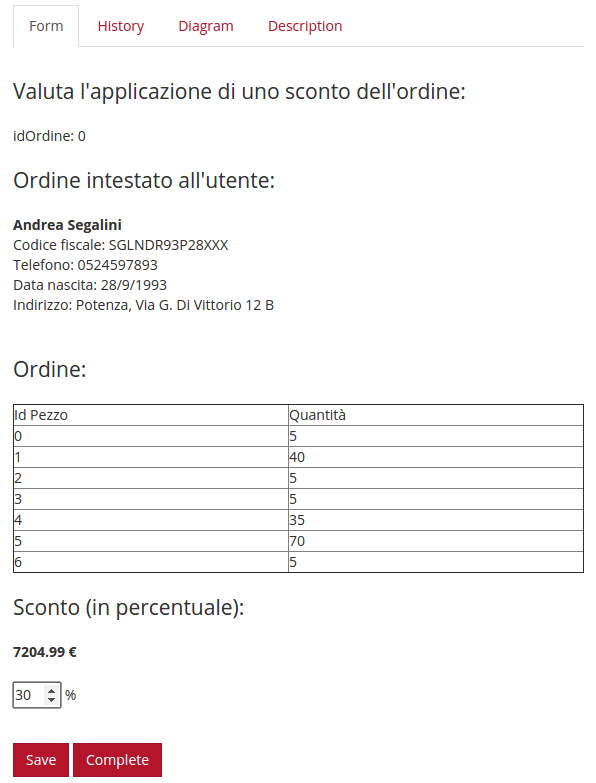
\includegraphics[width=8cm]{screen-form-sconto.png}
\label{fig:sconto}
\end{figure}

\subsection{Servizi aggiuntivi}
Descriviamo brevemente i servizi accessori che sono stati integrati nel nostro sistema.

\paragraph{Calcolo distanze geografiche.}
Per ogni prodotto richiesto, il magazzino che viene selezionato dal sistema per la spedizione
è quello che ha il prodotto disponibile e che è geograficamente più vicino alla sede del cliente.
Quindi, per rendere automatica tale procedura, si è sviluppata una funzione che prende in input
due città e ritorna la distanza tra queste in chilometri.
Per l'implementazione sono state usate API REST, facendo affidamento su Google, che mette a disposizione,
attraverso \emph{Google Maps API}, la possibilità di effettuare richieste REST, ottenendo cosi
informazioni dettagliate sul percorso preso in considerazione.
Un esempio concreto di richiesta, è il seguente:

\begin{lstlisting}
https://maps.googleapis.com/maps/api/distancematrix/json?origins=parma&destinations=pisa
\end{lstlisting}

Le risposte alle query di \emph{Google Maps Distance Matrix API} vengono restituite
nel formato indicato dal flag di uscita all'interno del percorso di richiesta dell'URL.
Infatti tale richiesta risponde in output con una pagina in formato JSON, contenente le informazioni di
percorso tra Bologna (settata come parametro d'esempio di origin) e Napoli
(che in questo caso è settato come destination):

\begin{lstlisting}
{
   "destination\_addresses" : [ "Napoli, Italia" ],
   "origin\_addresses" : [ "Bologna, Italia" ],
   "rows" : [
      {
         "elements" : [
            {
               "distance" : {
                  "text" : "575 km",
                  "value" : 575400
               },
               "duration" : {
                  "text" : "5 ore 34 min",
                  "value" : 20046
               },
               "status" : "OK"
            }
         ]
      }
   ],
   "status" : "OK"
}
\end{lstlisting}

Si noti che se si desidera estrarre dei valori dai risultati, in genere si necessita di analisi
e parsing JSON. Il parametro di interesse è \texttt{text}, contenuto nell'oggetto \texttt{distance},
ossia il valore testuale che contiene la distanza del percorso.

Siccome inizialmente la chiamata ``calcola distanza'' doveva essere effettuata all'interno di un
servizio Jolie, è stato introdotto un intermediario, sempre realizzato in Jolie, capace di effettuare le
chiamate REST al servizio di Google, esponendole poi attraverso web service SOAP.
La porta per effettuare richieste HTTP in Jolie è la seguente:

\begin{lstlisting}
outputPort DistanceMatrixService {
	Location: "socket://maps.googleapis.com:80/"
	Protocol: http { 
		.method = "get";
		.osc.default.alias = "maps/api/distancematrix/xml";
		.format = "xml"
	}
	Interfaces: DistanceMatrixInterface
}
\end{lstlisting}

All'interno della service task di Camunda, invece, la chiamata è stata effettuata direttamente
in Java senza passare per attraverso l'intermediario Jolie:

\begin{lstlisting}
URL url = new URL("https://maps.googleapis.com/maps/api/distancematrix/json?origins=" + 		
	      origine + "&destinations=" + destinazione);
HttpURLConnection conn = (HttpURLConnection) url.openConnection();
conn.setRequestMethod("GET");
conn.setRequestProperty("Accept", "application/json");		
BufferedReader br = new BufferedReader(new InputStreamReader((conn.getInputStream())));
\end{lstlisting}

\paragraph{Sistema bancario.}
ACME deve verificare, attraverso l'interazione con un sistema bancario, il pagamento degli importi
che gli vengono accreditati. Quindi è stato implementato un sistema elementare attraverso richieste REST.
Passando come parametro un identificativo del bonifico, risponde (in maniera casuale), tramite
un booleano, l'avvenuta o la mancata esecuzione del pagamento.
L'output contiene, poi, anche la somma pagata dal cliente che deve essere poi verificata
corrispondere all'importo richiesto.
 
\begin{lstlisting}
@Path("/bonifico")
public class Bonifico {
	
	public static boolean getRandomBoolean() { return Math.random() < 0.5; }
		
	@GET
	@Produces("application/json")
	public Response paytobank(@QueryParam("i") int i) throws JSONException {
		JSONObject jsonObject = new JSONObject();
		
		int price = 50;
		if(getRandomBoolean() == true){
			jsonObject.put("paycheck", true);
			jsonObject.put("price", price);
		} else{
			jsonObject.put("paycheck", false);
			jsonObject.put("price", price);
		}
		return Response.status(200).entity(jsonObject.toString()).build();
	}
}
\end{lstlisting}

Si noti che questa metodologia di pagamento è stata ipotizzata arbitrariamente,
non conoscendo le esatte funzionalità realmente offerte da una banca moderna.

\paragraph{Fornitore esterno.}
Il servizio di fornitore esterno è stato implementato con un'interfaccia di fatto
identica ai magazzini secondari. Tuttavia ciò non deve indurre a pensare che abbiano
una qualche relazione strutturale. Nel magazzino principale, infatti, c'è una netta
distinzione fra la gestione delle operazioni verso i magazzini secondari e di quelle
verso il fornitore esterno. La similarità fra essi è una pura semplificazione.

\section{Guida al deployment}
In questa sezione verranno illustrate le operazioni per la messa in opera di tutto il sistema.
\`E richiesto:
\begin{itemize}
	\item Java Development Kit 7. \\
		  Nel progetto si è scelto di usare OpenJDK.
	\item Un application server JBoss AS 7.4.0. \\
		  In particolare, poi, nel progetto si è adoperato
		  quello distribuito da Camunda \footnote{Pagina di download \url{www.camunda.org/download}}.
	\item Jolie Language. \\
		  Nel nostro caso, si è adottata la versione 1.4.1 \footnote{Sito web \url{www.jolie-lang.org}}.
	\item Apache Maven. \\
		  Per i nostri esperimenti, si è installata la versione 3.3.3.
	\item Un accesso ad internet per accedere ai web services di Google.
\end{itemize}


\subsection{Deployment del magazzino principale}
La struttura generale dell'applicativo può essere sintetizzata nel seguente albero:

\begin{forest}
  for tree={
    font=\ttfamily,
    grow'=0,
    child anchor=west,
    parent anchor=south,
    anchor=west,
    calign=first,
    edge path={
      \noexpand\path [draw, \forestoption{edge}]
      (!u.south west) +(7.5pt,0) |- node[fill,inner sep=1.25pt] {} (.child anchor)\forestoption{edge label};
    },
    before typesetting nodes={
      if n=1
        {insert before={[,phantom]}}
        {}
    },
    fit=band,
    before computing xy={l=15pt},
  }
[magazzino\_principale
    		[magazzinoPrincipale.ol \textbf{Applicazione Jolie service server}]
    		[creaDBMagazzinoPrincipale.ol 
    		 \textbf{Crea il database "db/DB\_magazzinoPrinc"}]
    		[popolaDBMagazzinoPrincipale.ol 
    		 \textbf{Popola il database con dati di prova}]
  	[lib
  		[hsql.jar \textbf{DBMS hsql}]
   	]
   	[db
		[... \textbf{File del DB hsql "DB\_magazzinoPrinc"}]   	
   	]
]
\end{forest}

\`E fondamentale che le directory \texttt{interfacce} e \texttt{magazzino\_principale}
(che, ricordiamo, possiede anche un magazzino secondario)
siano contenute nella stessa cartella:

\begin{forest}
  for tree={
    font=\ttfamily,
    grow'=0,
    child anchor=west,
    parent anchor=south,
    anchor=west,
    calign=first,
    edge path={
      \noexpand\path [draw, \forestoption{edge}]
      (!u.south west) +(7.5pt,0) |- node[fill,inner sep=1.25pt] {} (.child anchor)\forestoption{edge label};
    },
    before typesetting nodes={
      if n=1
        {insert before={[,phantom]}}
        {}
    },
    fit=band,
    before computing xy={l=15pt},
  }
[root
	[interfacce
  		[dataTypes.iol \textbf{Definizione struttura messaggi XML}]
  		[interfacciaMagazzinoPrincipale.iol \textbf{Definizione operation magazzino principale}]
  		[interfacciaMagazzinoSecondario.iol \textbf{Definizione operation magazzino secondario}]
  		[interfacciaFornitore.iol \textbf{Definizione operation fornitore esterno}]
  	]
  	[magazzino\_principale]
  	[magazzino\_secondario1]
]
\end{forest}

Le operazioni per il deployment del magazzino principale possono essere riassunte nei seguenti punti:
\begin{enumerate}
	\item Configurazione del file \texttt{magazzinoPrincipale.conf}, in cui vengono
		  impostati i parametri del database (si consiglia di lasciare inalterati i
		  parametri i default).
	\item Creazione del database tramite l'esecuzione di un programma Jolie:
\begin{lstlisting}
$ jolie creaDBmagazzinoPrincipale.ol
\end{lstlisting}
	\item (Opzionale) Popolamento database con dati di prova:
\begin{lstlisting}
$ jolie popolaDBmagazzinoPrincipale.ol
\end{lstlisting}
	\item Avvio del web service server del magazzino principale:
\begin{lstlisting}
$ jolie magazzinoPrincipale.ol
\end{lstlisting}
\end{enumerate}
Con le impostazioni di default, il magazzino principale ascolta all'indirizzo
\texttt{localhost:8000}. Per modificare la porta d'ascolto è necessario cambiare
l'attributo nel file di configurazione e nel sorgente del magazzino principale.
Questo avviene dal momento che Jolie non permette di settare dinamicamente la location d'ascolto.
In standard output viene stampato il log del servizio con alcune informazioni utili per
eventuale debugging.

\subsection{Deployment del magazzino secondario}
La struttura generale dell'applicativo può essere sintetizzata nel seguente albero:

\begin{forest}
  for tree={
    font=\ttfamily,
    grow'=0,
    child anchor=west,
    parent anchor=south,
    anchor=west,
    calign=first,
    edge path={
      \noexpand\path [draw, \forestoption{edge}]
      (!u.south west) +(7.5pt,0) |- node[fill,inner sep=1.25pt] {} (.child anchor)\forestoption{edge label};
    },
    before typesetting nodes={
      if n=1
        {insert before={[,phantom]}}
        {}
    },
    fit=band,
    before computing xy={l=15pt},
  }
  	[magazzino\_secondario
    		[magazzinoSecondario.ol \textbf{Applicazione Jolie service server}]
    		[creaDBMagazzinoSecondario.ol 
    		 \textbf{Crea il database "db/DB\_magazzinoSec"}]
    		[popolaDBMagazzinoSecondario.ol 
    		 \textbf{Popola il database con dati di prova}]
  	[lib
  		[hsql.jar \textbf{DBMS hsql}]
   	]
   	[db
		[... \textbf{File del DB hsql "DB\_magazzinoSec"}]   	
   	]
   	]
\end{forest}

Anche in questo caso è necessario che le directory \texttt{magazzino\_secondario} e
\texttt{interfacce} siano contenute nella stessa cartella.

Le operazioni per il deployment del magazzino secondario si possono riassumere nei seguenti punti:
\begin{enumerate}
	\item Configurazione del file \texttt{magazzinoSecondario.conf}, in cui vengono
		  impostati i parametri del database (anche in questo caso, si consiglia di lasciare inalterati i
		  parametri i default).
	\item Creazione del database tramite l'esecuzione di un programma Jolie:
\begin{lstlisting}
$ jolie creaDBmagazzinoSecondario.ol
\end{lstlisting}
	\item (Opzionale) Popolamento del database con dati di prova (appositi per il magazzino 
		  $n$-esimo, nell'esempio sotto si fa riferimento al secondo):
\begin{lstlisting}
$ jolie popolaDBmagazzinoSecondario2.ol
\end{lstlisting}
	\item Avvio del web service server del magazzino secondario:
\begin{lstlisting}
$ jolie magazzinoSecondario.ol
\end{lstlisting}
\end{enumerate}

Per aggiungere un nuovo magazzino a tutto il sistema, è necessario creare una copia
dell'applicativo di un magazzino secondario e modificare il file di configurazione,
specificando l'id corrispondente alla nuova entità che si viene a creare. Ricordiamo
che è necessario modificare anche l'input port nel sorgente \texttt{magazzinoSecondario.ol}
con la location desiderata.
In questa implementazione del sistema è necessario registrare nel database del magazzino
principale un nuovo record nella tabella \texttt{Magazzini}, in modo che possa essere
automaticamente considerato nell'esecuzione delle operazioni di ACME.

\subsection{Deployment del fornitore esterno}
La struttura generale del fornitore esterno può essere sintetizzata nel seguente albero:

\begin{forest}
  for tree={
    font=\ttfamily,
    grow'=0,
    child anchor=west,
    parent anchor=south,
    anchor=west,
    calign=first,
    edge path={
      \noexpand\path [draw, \forestoption{edge}]
      (!u.south west) +(7.5pt,0) |- node[fill,inner sep=1.25pt] {} (.child anchor)\forestoption{edge label};
    },
    before typesetting nodes={
      if n=1
        {insert before={[,phantom]}}
        {}
    },
    fit=band,
    before computing xy={l=15pt},
  }
  	[fornitore\_esterno
    		[fornitore.ol \textbf{Applicazione Jolie service server}]
    		[creaDBMagazzinoFornitore.ol 
    		 \textbf{Crea il database "db/DB\_fornitore"}]
    		[popolaDBMagazzinoFornitore.ol 
    		 \textbf{Popola il database con dati di prova}]
  	[lib
  		[hsql.jar \textbf{DBMS hsql}]
   	]
   	[db
		[... \textbf{File del DB hsql "DB\_magazzinoSec"}]   	
   	]
   	]
\end{forest}

Ancora una volta, è necessario che le directory \texttt{fornitore\_esterno} e
\texttt{interfacce} siano contenute nella stessa cartella, come spiegato sopra.

Le operazioni per il deployment del fornitore esterno si possono riassumere nei seguenti punti:
\begin{enumerate}
	\item Configurazione del file \texttt{fornitore.conf}, in cui vengono
		  impostati i parametri del database (anche in questo caso, si consiglia di lasciare
		  inalterati i valori di default).
	\item Creazione del database tramite l'esecuzione di un programma Jolie:
\begin{lstlisting}
$ jolie creaDBmagazzinoFornitore.ol
\end{lstlisting}
	\item (Opzionale) Popolamento del database con dati di prova:
\begin{lstlisting}
$ jolie popolaDBmagazzinoFornitore.ol
\end{lstlisting}
	\item Avvio del web service server del fornitore esterno:
\begin{lstlisting}
$ jolie magazzinoFornitore.ol
\end{lstlisting}
\end{enumerate}

Come per i magazzini secondari, il fornitore esterno deve essere aggiunto all'interno
della tabella \texttt{Magazzini} nel database del magazzino principale.

\subsection{Deployment dell'amministrazione (processo Camunda)}
Il deployment avviene mediante l'esportazione dell'applicazione in un archivio \texttt{war},
collocato poi nell'apposito application server. Per ottenerlo, aperto un terminale e collocatisi
nella directory del progetto, è sufficiente eseguire l'istruzione:
\begin{lstlisting}
$ mvn clean package
\end{lstlisting}
Il \texttt{war} generato è presente nella directory \texttt{target}.
Notiamo come nella consegna siano presenti due diverse applicazioni per l'implementazione
del business process, a causa di alcuni problemi che saranno discussi dettagliatamente in
sezione \ref{conclusioni}.
\texttt{selling-cycles-no-ws-start-working} è l'applicativo che non consente l'avvio, tramite
messaggio, del processo Camunda, ma permette l'esecuzione di tutti i task necessari alla
corretta conclusione del processo. L'altro, al contrario, consente al processo Camunda di
avviarsi con successo, ma presenta problematiche relativamente a


\section{Conclusioni e problematiche} \label{conclusioni}
La progettazione e realizzazione (tramite paradigma SOA) del sistema di ACME
non è stata esente da problemi. In primo luogo, il linguaggio
Jolie si presta bene all'esposizione di servizi, ma risulta molto macchinoso
nella programmazione general purpose, a causa dell'assenza del concetto di ``funzione'',
sostituito dalle ``operations'', e dello scope dinamico che ci ha costretto
ad usare soluzioni non sempre eleganti. Segnaliamo inoltre alcuni problemi
riscontrati durante lo sviluppo, nel momento in cui è stato necessario
far comunicare fra loro entità realizzate con tecnologie differenti:
\begin{itemize}
	\item  Jolie ha dei problemi con gli ``a capo'' \texttt{<CR>} 
		   che client come SoapUI inseriscono nei messaggi XML.
		   L'opzione \texttt{dropRootValue} risolve il problema \textbf{solo} per la radice del messaggio;
		   in presenza quindi di tipi strutturati non primitivi la problematica persiste.
		   Per questo, in programmi con messaggi semplici (come la calcolatrice vista a lezione)
		   ciò non accade. Nel nostro caso, invece, a quanto pare 
		   è presente un bug non ancora fixato che ne impedisce il corretto funzionamento.
		   Riportiamo il link alla discussione originale
		   \footnote{Discussione bug \url{www.github.com/jolie/jolie/issues/44}}.
	\item \`E stato riscontrato che, realizzando un client Java per un servizio Jolie,
		  le operation ``oneway'' bloccano l'esecuzione del codice. Questo problema non
		  è stato approfondito e non è noto se sia dovuto alla generazione automatica
		  a partire dal WSDL oppure se si tratta di una vera e propria incompatibilità tra Java e Jolie.
\end{itemize}

In teoria, sarebbe stato necessario usare JBoss poiché supporta le primitive che consentono,
ricevendo un'invocazione all'interno di un web service, di avviare un processo Camunda. Tuttavia
in questo application server non si è riusciti ad effettuare le chiamate ai servizi Jolie
necessarie per il completamento di tutte le operazioni. Il problema sembra dipendere
dalle mancate dipendenze richieste dal web service client auto-generato a partire dal WSDL
con Apache CXF. Alcuni test ci hanno permesso di identificare il problema
proprio nell'auto-generazione a partire da quel determinato WSDL ottenuto dal codice Jolie.
Le chiamate verso altri server, infatti, funzionano correttamente.
Nel codice presentato, questo problema è stato aggirato utilizzando il web server Tomcat, il quale,
pur senza realizzare l'auto-avvio del processo Camunda a seguito di un messaggio,
permette di simulare l'esecuzione del processo business.

Concludendo, tramite la realizzazione e lo studio delle attività di ACME, è stato possibile
apprezzare a pieno i vantaggi del paradigma service-oriented. Contemporaneamente,
siamo rimasti alquanto delusi da come gli standard risentano delle diverse implementazioni,
portando talvolta a fastidiose incompatibilità che rappresentano un'incongruenza rispetto alla 
suddetta filosofia.


%----------------------------------------------------------------------------------------
%	ARTICLE CONTENTS
%----------------------------------------------------------------------------------------

%\printbibliography

\end{document}
